\section{Diagrama de clases del sistema de mensajer\'ia}

El siguiente diagrama de clases muestra las clases, con sus respectivos argumentos y m\'etodos, que se pretende implementar para el dise\~no de nuestro sistema de mensajer\'ia. 

Podemos observar que se hace uso de MVC (Model-View-Control), mediante el cual pretendemos agrupar los componentes de la aplicaci\'on en tres niveles l\'ogicos: modelo, vista y controlador.

En el modelo se pretende representar la informaci\'on que el sistema manipulara.

La vista generar\'a una representaci\'on visual del Modelo y muestrar\'a los datos al Contacto, permitiendo que \'este interactuel con el sistema.

Y finalmente el controlador que ser\'a quien responda a eventos o acciones invocadas por el Contacto. 



%	\begin{figure}[htbp!]
%		\centering
%			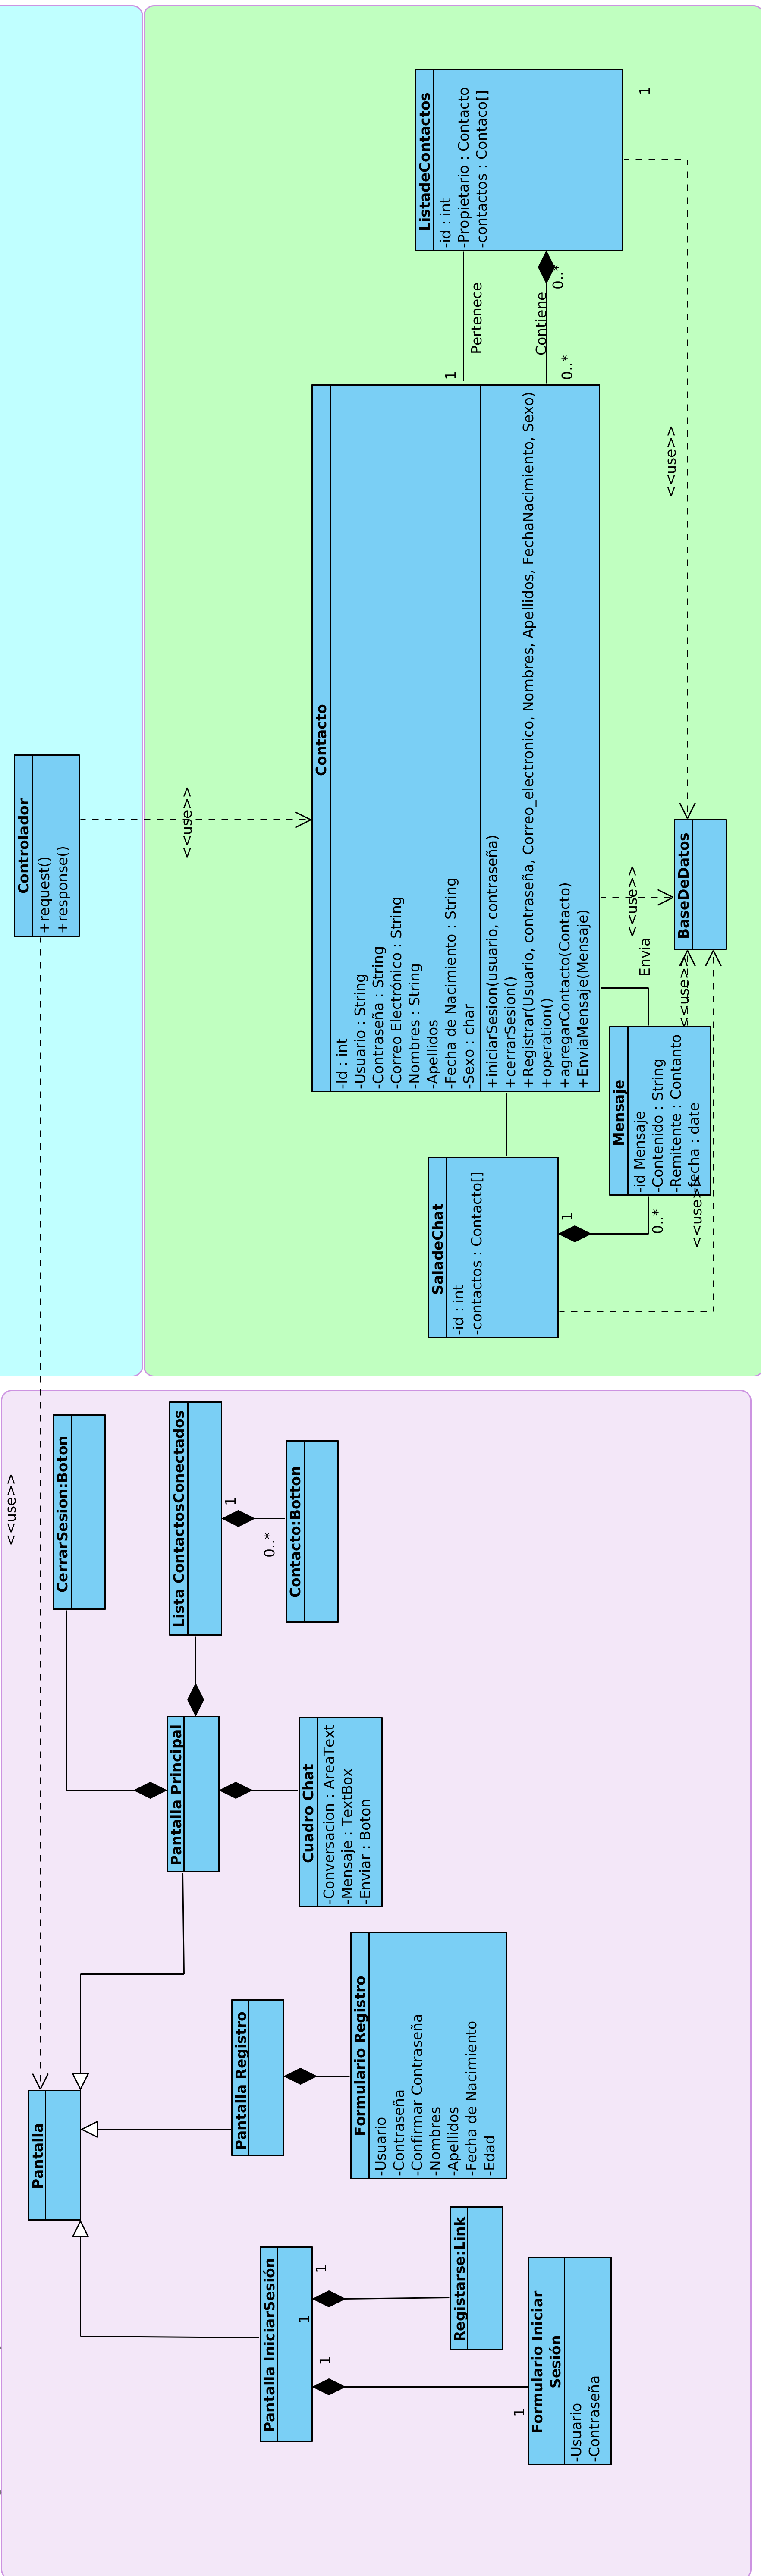
\includegraphics[width=12cm, height=20cm]{images/Diagramas/dclases}
%		\caption{Diagrama de Clases del sistema de mensajer\'ia.}
%	\end{figure}
	
	\begin{figure}[htbp!]
		\centering
			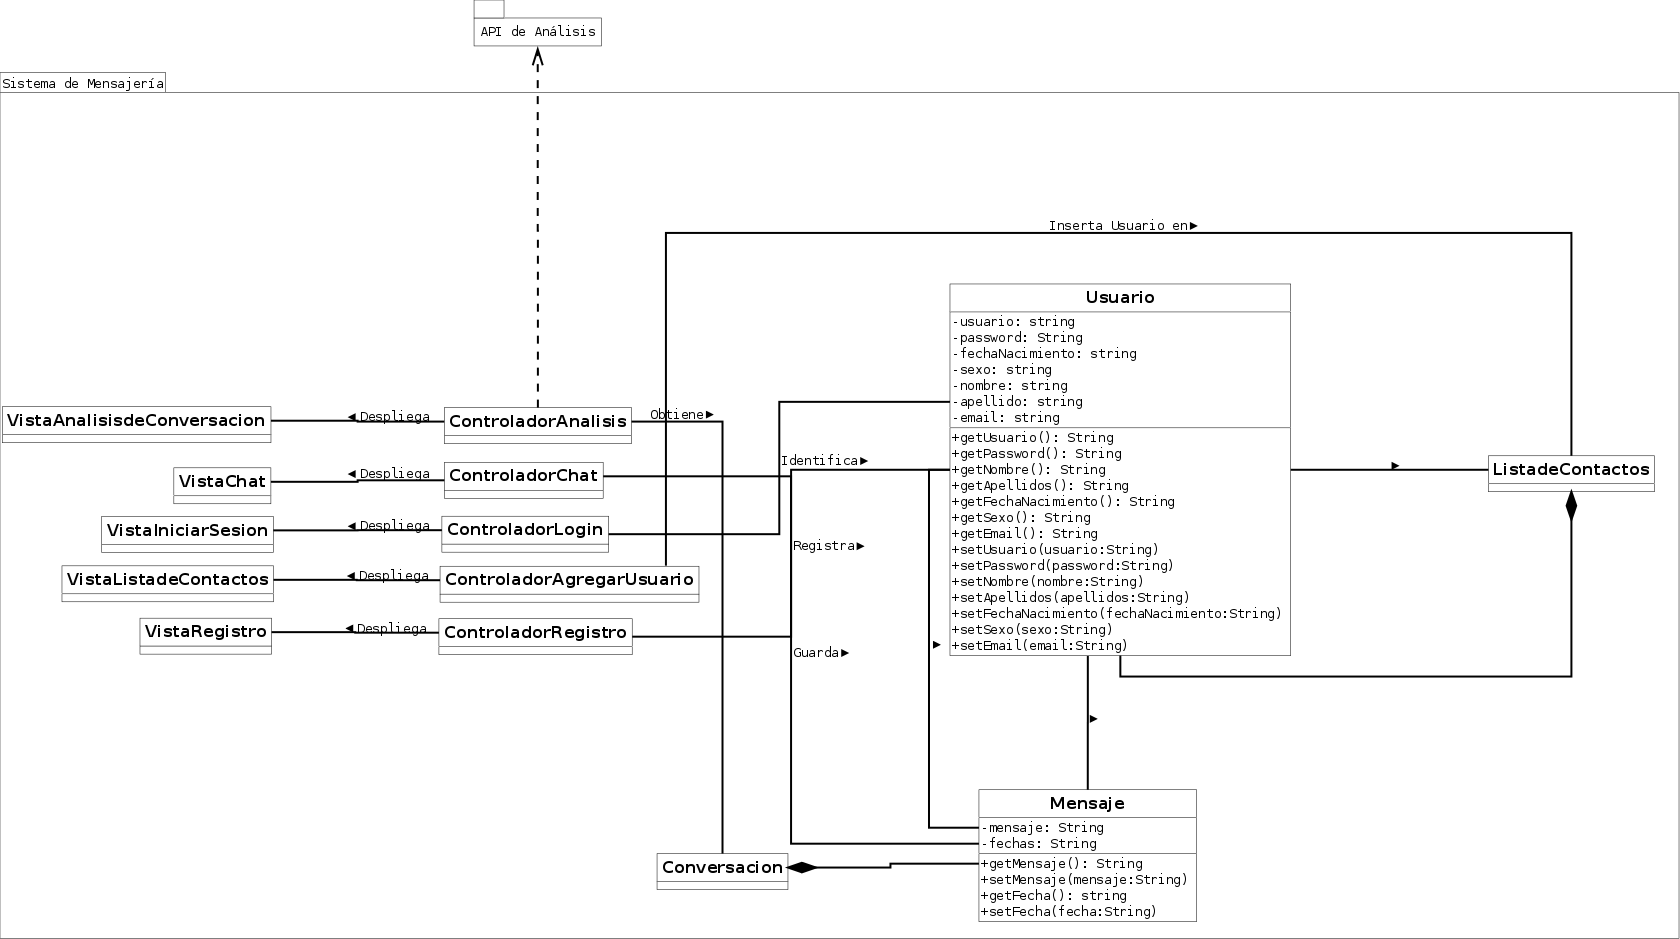
\includegraphics[width=18cm, height=13cm]{images/Diagramas/ddclases}
		\caption{Diagrama de Clases del sistema de mensajer\'ia.}
	\end{figure}
	
	

	
	\pagebreak